\chapter{Design}
\label{chap:Design}
In this chapter I will look into designing the system, starting out with how the database should look in order for it to be able to store the data in a way that allows me to easily access it again, while reducing redundant data stored.

After the database I will get into how the system will be structured, which includes explaining the model that I will be following. Finally I will give a short explanation of some of the patterns I will be following, and why they are useful for a system such as this one.

\section{Database}
\label{sec:Database}
The design of the database will look on many points similar to the domain model in figure~\ref{fig:domain_model}. This is because on a lot of the points in this system the domain model can be saved directly to the database. I have of course had to make some adjustments, as can be seen in figure~\ref{fig:Database model}.

\begin{figure}
  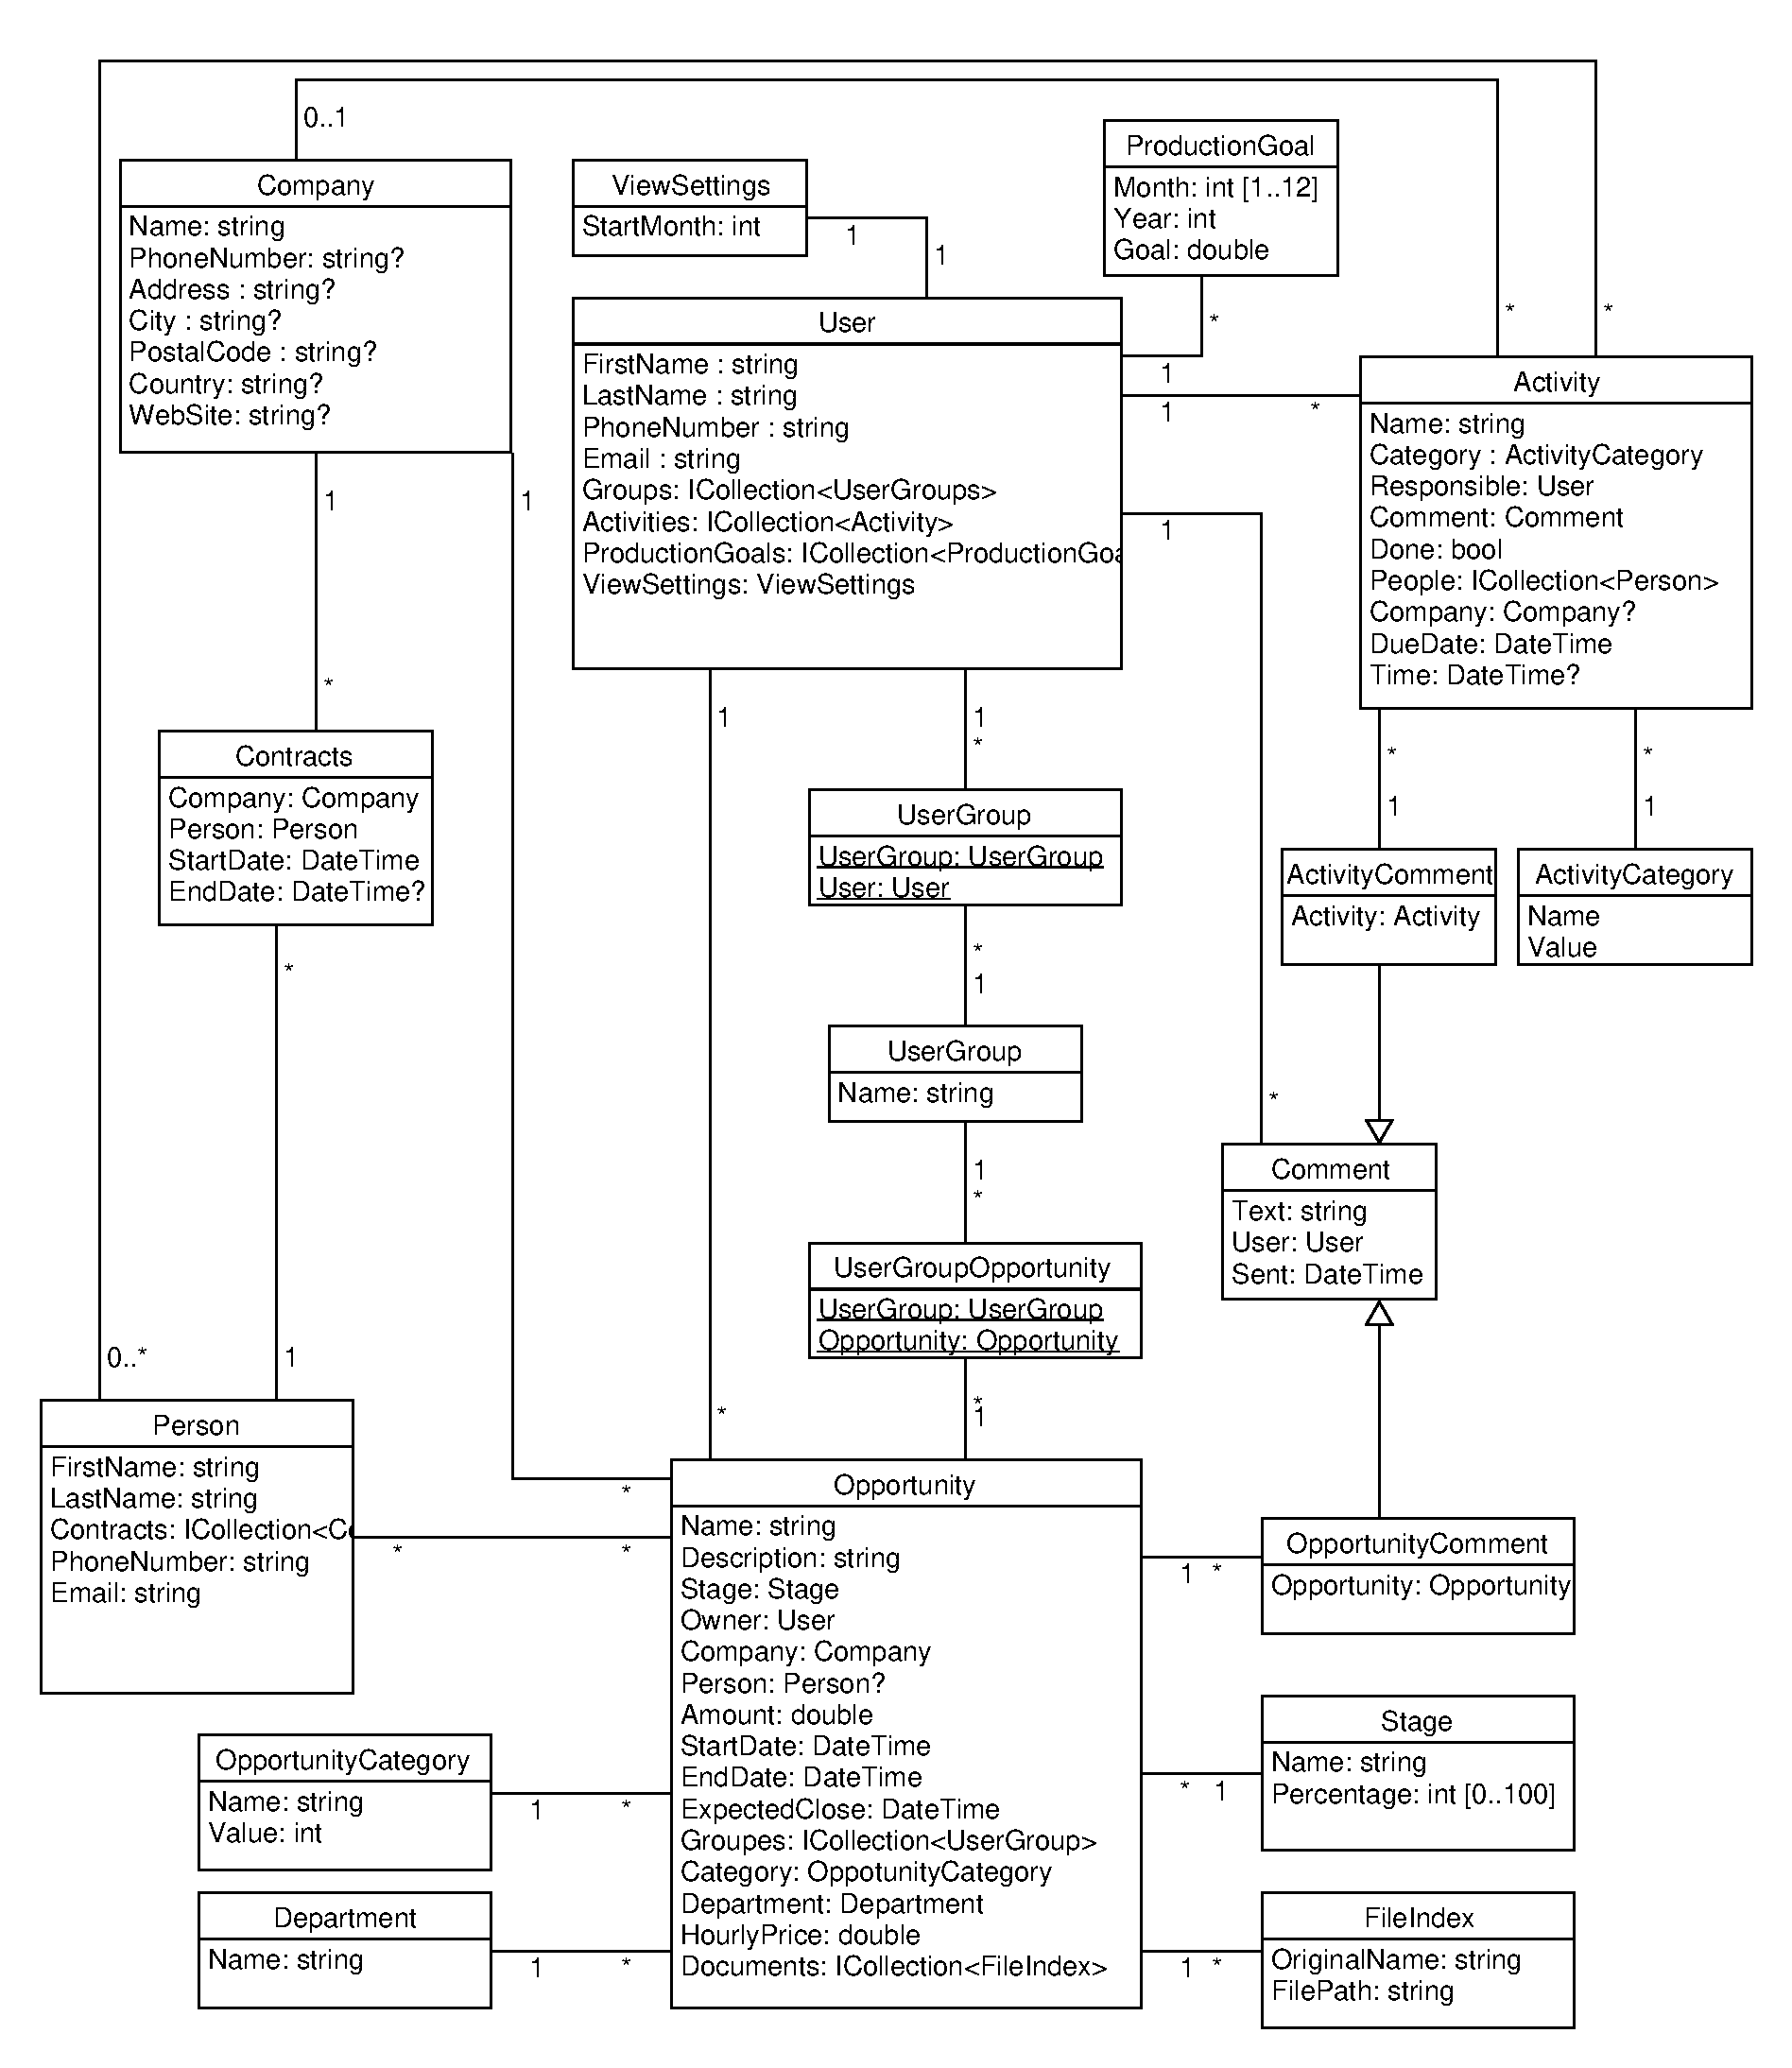
\includegraphics[width=\textwidth]{db_model}
  \caption{Database model}
  \label{fig:Database model}
\end{figure}

For the entities with many-to-many relations I have chosen not to show the linking tables as it makes it harder to read, and the tables unless they are actually drawn as is the case with EndedContracts, they will have a primary key set of the two foreign keys of the referred tables.

One thing that will be noticed is that now I have datatypes on the model. This is because this model is meant to describe what is in the database.

The design is in NF1\footnote{First Normal Form} because I do not have any rows containing any duplicate information, such as a company having a column for all their workers, instead the workers are separated out into a different table\cite[p.~430]{DB_systems}, the same is true for a user and their goals and user groups, instead of having a list of them in the table itself, I have it separated out into different tables.

It is also in NF2\footnote{Second Normal Form} because none of the properties of any of the tables are functionally dependent on anything other than the primary key of the table\cite[p.~434]{DB_systems}. In this case I have not added the primary key to the tables since they will all be called Id as per convention of the entity framework, and I will be giving them an integer as the datatype. In cases where properties are underlined in the model, it means that I don't have an id column, but instead is using the underlined properties as my primary key.

The next normal form would be the third normal form. I have come to the conclusion that it is not worth the hassle of perusing this last part as the goal with it is to reduce redundant data to even greater extent, which would mean I would have to move the location based fields of Company out into a separate table in order for me to remove the transitive dependency\cite[p.~436]{DB_systems} there is between the city, address, and postal code, as well as the country. The reason for not pursuing this is that I have deemed the gain not worth it, since it would bind all locations in the same area together, and the users may not be interested in this, since if they then change the postal code or city name of one company, the rest that is located in the same place will follow.

Some people argue that nulls should be allowed and others that there should be no nulls in a database\cite{stackexchange:db:nullfields}, and I do see the reasoning of their arguments, generally that you cannot know what null represents, it could mean the absence of data, purposefully or something else.

One argument is if there is a null value in eg. an integer could mean both null and unknown. A solution to having null values in ones database could be to split it into several tables, one for each potential missing value. I have decided not to do this, since it would make the diagram harder to read, and the database harder to comprehend. Another reason I have chosen not to get rid of all nulls is that I have decided that if a value can be and is null. Then it means that value is not meant to be there. So I will not interpret null as anything but the absence of data.

As an example if I look at the table contracts, the end date can be null, which would mean that there is no end date, and hence the contract is not terminated. If there were an end date however then the termination has been set, maybe in the future, or maybe in the past, that is dependent on the value, but it means that the time of the ended relationship with the company is known.

This forces me to still think about if I should allow a value to e null or not, without forcing me out of the possibility which is why I have chosen that solution.

In the model I have a datatype that is not really related to the database as much as it is to the programming language, the \textit{ICollection<T>} is a type the entity framework uses to create an inverse navigation property, and the only reason I have it in this model is that it gives an idea that it should be possible to navigate in the inverse direction of the actual link.

\section{System structure}
\label{sec:System structure}
The structure of the system follows the onion architecture\cite{onion_architecture}, which means that it is build up of layers like it can be seen on figure~\ref{fig:Onion architecture}.

\begin{figure}[h]
  \centering
  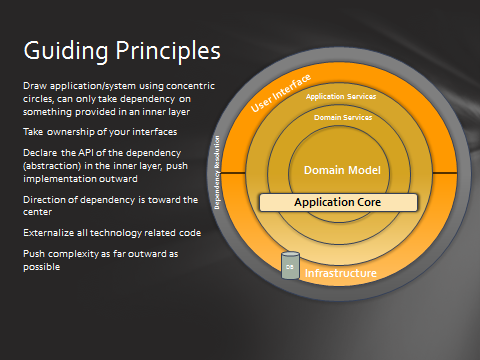
\includegraphics{onion_model}
  \caption[Onion architecture]{Onion architecture\protect\footnotemark}
  \label{fig:Onion architecture}
\end{figure}
\footnotetext{Source: http://www.matthidinger.com/images/www\_matthidinger\_com/Windows-Live-Writer/ff0d136aee1f\_88EA/image\_2.png}

In figure~\ref{fig:structure} the setup that my project will follow is illustrated. As can be seen I have three core projects, one for each of the core layers of the model, and outside this I have an infrastructure layer, which is responsible for talking to the database. The way the outer most layers then work is by using the interfaces that is defined in \textit{Core.DomainServices}. These interfaces describe how the application can access the data however it is stored.

\begin{figure}[h]
  \centering
  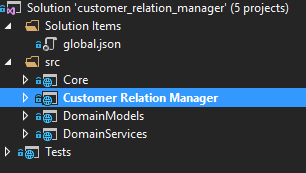
\includegraphics{structure}
  \caption{Structure of the system}
  \label{fig:structure}
\end{figure}

I use injection to allow for easier testing, and lower dependency between the classes. This means that in the project \textit{customer\_relations\_manager} which is where the controllers the users will be calling is implemented, take interfaces for the repositories defined in \textit{Core.DomainServices}. The injection system then is set up to inject the classes from \textit{Infrastructure.DataAccess} that implement the interfaces.

The \textit{Core.ApplicationServices} project is there in the case that I need a service that is not related to accessing data from the data store, but instead doing something else.

Finally the inner most layer is the classes describing the data that is stored in my case in a database the name of this project is \textit{Core.DomainModels}. Their job is to describe how the data looks in the database, and they are used for making the database first migrations.

The \textit{UnitTests} project is on the same level as \textit{customer\_relations\_manager}, which means that it is allowed to see everything in the project, allowing it to test it all.

The goal with all this separation is to both make it easier to swap out parts of the project without too much hassle, and to be able to reuse parts, in case I want to do something similar in the future. It does however also force us to not have an uncontrollable mess of dependencies, since the domain models are never allowed to know anything other than them selves, and the data access layer cannot say anything about how the data will look in the end, only find and filter on it.

\section{Patterns}
\label{sec:Patterns}

\subsection{Dependency injection}
\label{sub:Dependency injection}
In order for us to reduce coupling in the code I can use dependency injection. Dependency injection is the idea of letting the caller instantiate all of our dependencies instead of creating them in the class where I need it.

There are several advantages of this, one of which is that I can easily isolate a single unit of the program for testing, and then do unit testing on that single unit. I can then make mocks of all of its dependencies, and therefore know exactly how the different dependencies will react depending on my test code\cite{dependency_injection}.

A way to reduce coupling even further is to instead of depending on a specific class. I can depend on an interface, which will allow me to only rely on a specific set of methods of the class, and then the user can decide what implementation they finds best suited.

\subsection{Repository pattern}
\label{sub:Repository pattern}
The objective with the repository pattern is to separate the business logic away from the data access logic, resulting in the business logic not caring about where the data comes from, as it will just call a repository, and expect some data to come back.

An advantage of this pattern is that the developer implementing the business logic can have a mocked implementation of the repository, that just uses some form of local storage. It allows the developers to delay the decision of where to store the data, as the repository does not have to be implemented to access a database, but it could read from a file, request a web service, or something else\cite{repository_pattern}.

\subsection{Unit of work pattern}
\label{sub:Unit of work pattern}
A pattern that works well with the repository pattern, that is described in section~\ref{sub:Repository pattern}, is the unit of work pattern. The goal of this pattern is to group up execution of operations that has an impact on the data store. In cases where I just read out from the database I may not need it, but in cases where I change data it makes sense to be in a state where I either do all of the intended operations or none of them.

The problem that the unit of work pattern solves is that if I am updating some object, which includes the deletion of some data, I want to make sure that if something fails later on after I have done the delete, so that the creation was not done, the delete operation is abandoned, and I have not damaged my data model\cite{uow}.

\section{Chapter summary}
\todo{Summarize}
